\chapter{RNN}
\setlength{\parskip}{6pt}
\begin{enumerate}
	\item RNN原理	
	\begin{figure}[h]
		\centering
		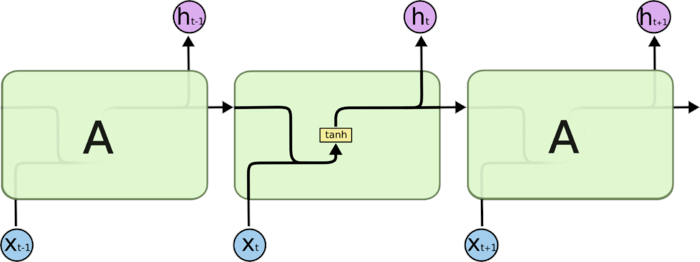
\includegraphics[width=1\textwidth]{./Tex_files/rnn1.jpg}
		\caption{RNN原理图}
		\label{wolf}
	\end{figure}
	基础的神经网络只在层与层之间建立了权连接,RNN最大的不同之处就是在层之间的神经元间也建立了权的连接。
	\begin{figure}[h]
		\centering
		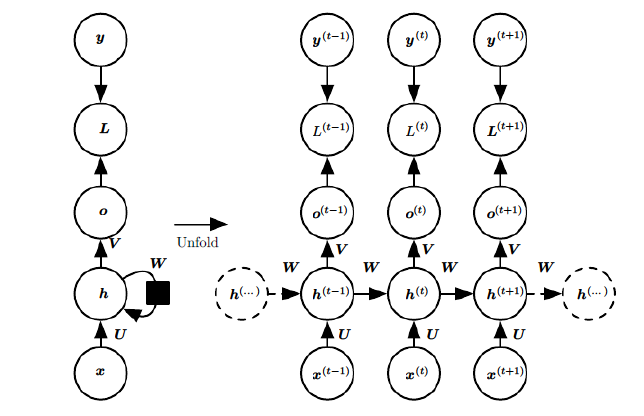
\includegraphics[width=1\textwidth]{./Tex_files/rnn2.png}
		\caption{RNN展开}
		\label{wolf}
	\end{figure}	
	其中,$x$是输入,$h$是隐含单元,$o$是输出,$L$是损失函数,$y$是训练集的标签。$V,W,U$是权值。\\
	对于$t$时刻的前向传播算法:
	\begin{flalign}
		h^{(t)}=\phi(Ux^{(t)}+Wh^{(t-1)}+b)
	\end{flalign}
	其中$\phi()$为激活函数,$b$为偏置。\\
	t时刻的输出:
	\begin{flalign}
		o^{(t)}=Vh^{(t)}+c
	\end{flalign}	
	最终模型的预测输出为:
	\begin{flalign}
		\hat y^{(t)}=\theta(o^{(t)})
	\end{flalign}
	其中$\theta$为激活函数,通常RNN用于分类,故这里一般用softmax函数。\\
	第$t$层的隐含状态$h_t$编码了序列中前$t$个输入的信息,可以通过当前的输入$x_t$和上一层神经网络的状态$h_{t-1}$计算得到;最后一层的状态编码$h_T$编码了整个序列的信息。\\
	通过最小化损失误差(即输出的y与真实类别之间的距离),我们可以不断训练网络。
	\item RNN的训练方法————BPTT
	BPTT(back-propagation through time)算法是常用的训练RNN的方法,其实本质还是BP算法,只不过RNN处理时间序列数据,所以要基于时间反向传播,故叫随时间反向传播。BPTT的中心思想和BP算法相同,沿着需要优化的参数的负梯度方向不断寻找更优的点直至收敛。综上所述,BPTT算法本质还是BP算法,BP算法本质还是梯度下降法,那么求各个参数的梯度便成了此算法的核心。
	\begin{figure}[h]
		\centering
		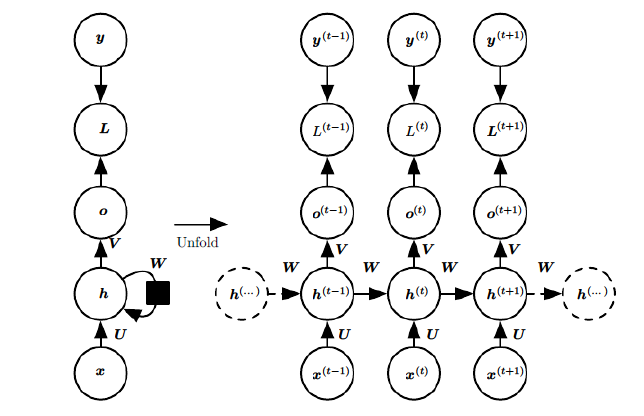
\includegraphics[width=1\textwidth]{./Tex_files/rnn2.png}
		\caption{RNN展开}
	\end{figure}
	在某个时刻对$W$或是$U$的偏导数,需要追溯这个时刻之前所有时刻的信息。
	\begin{flalign}
		\frac{\partial L^{(t)}}{\partial W}=\sum_{k=0}^{t}\frac{\partial L^{(t)}}{\partial o^{(t)}}\frac{\partial o^{(t)}}{\partial h^{(t)}}(\prod_{j=k+1}^{t}\frac{\partial h^{(j)}}{\partial h^{(j-1)}})\frac{\partial h^{(k)}}{\partial W}\\
		\frac{\partial L^{(t)}}{\partial U}=\sum_{k=0}^{t}\frac{\partial L^{(t)}}{\partial o^{(t)}}\frac{\partial o^{(t)}}{\partial h^{(t)}}(\prod_{j=k+1}^{t}\frac{\partial h^{(j)}}{\partial h^{(j-1)}})\frac{\partial h^{(k)}}{\partial U}
	\end{flalign}
	我们会发现累乘会导致激活函数导数的累乘,进而会导致“梯度消失“和“梯度爆炸“现象的发生。如果取sigmoid函数作为激活函数的话,那么必然是一堆小数在做乘法,结果就是越乘越小。随着时间序列的不断深入,小数的累乘就会导致梯度越来越小直到接近于0,这就是“梯度消失“现象。\\
	解决“梯度消失“的方法主要有:
	\begin{enumerate}
		\item 选取更好的激活函数(relu)	
		\item 改变传播结构(LSTM)
	\end{enumerate}
	\item LSTM
	\begin{figure}[h]
		\centering
		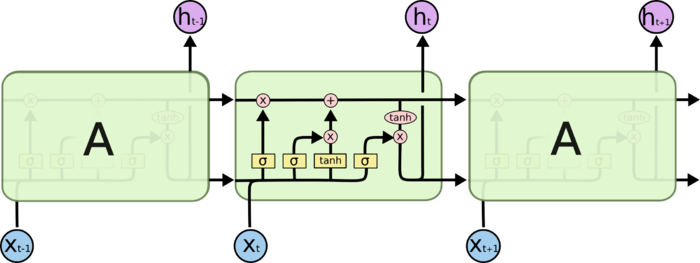
\includegraphics[width=1\textwidth]{./Tex_files/lstm1.png}
		\caption{LSTM原理}
	\end{figure}
	\\
	LSTM 有通过精心设计的称作为“门”的结构来去除或者增加信息到细胞状态的能力。门是一种让信息选择式通过的方法。他们包含一个 sigmoid 神经网络层和一个 pointwise 乘法操作。Sigmoid 层输出 0 到 1 之间的数值,描述每个部分有多少量可以通过。0 代表“不许任何量通过”,1 就指“允许任意量通过”!\\
	\begin{enumerate}
		\item 遗忘门\\
		在LSTM中第一步是我们决定会从细胞状态中丢弃什么信息,该门会读取$h_{t-1}$和$x_t$,输出一个在0到1之间的数据给每个在细胞状态$C_{t-1}$中的数字。1表示完全保留,0表示完全舍弃。
		\begin{figure}[h]
			\centering
			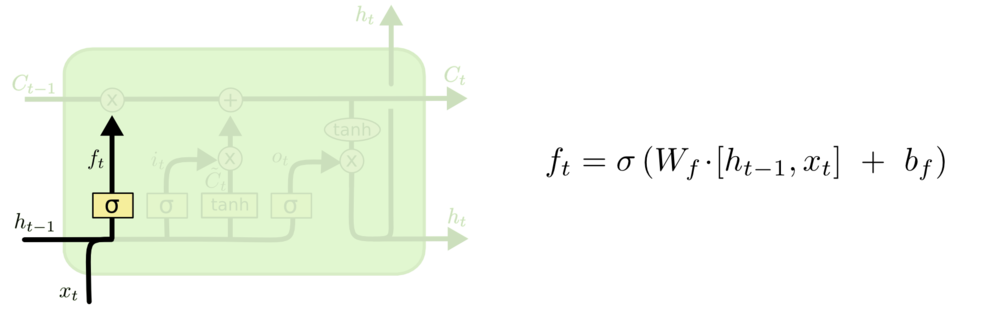
\includegraphics[width=1\textwidth]{./Tex_files/lstmforget.png}
			\caption{LSTM遗忘门}
		\end{figure}
		\item 输入门\\
		下一步是确定什么样的新信息被存放在细胞状态中。这里包含两个部分。第一,sigmoid称 “输入门层” 决定什么值我们将要更新。然后,一个tanh层创建一个新的候选值向量,$\tilde{C}_t$,会被加入到状态中。下一步,我们会讲这两个信息来产生对状态的更新。
		\begin{figure}[h]
			\centering
			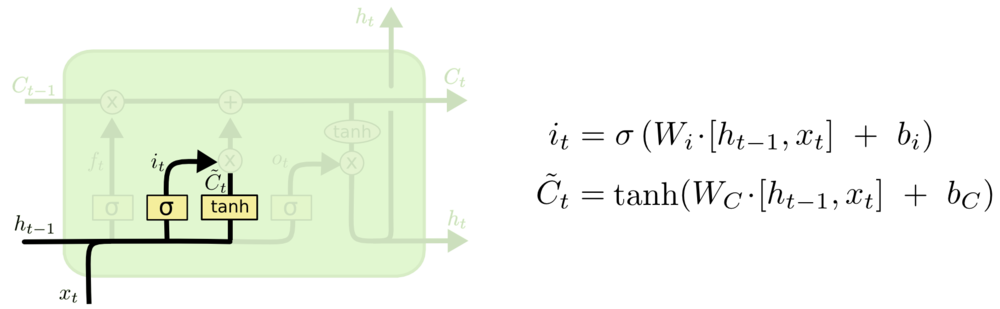
\includegraphics[width=1\textwidth]{./Tex_files/lstminput.png}
			\caption{LSTM输入门}
		\end{figure}
		\item 更新状态
		我们把旧状态与$f_t$相乘,丢弃掉我们确定需要丢弃的信息。接着加上$i_t * \tilde{C}_t$。这就是新的候选值,根据我们决定更新每个状态的程度进行变化。
		\begin{figure}[h]
			\centering
			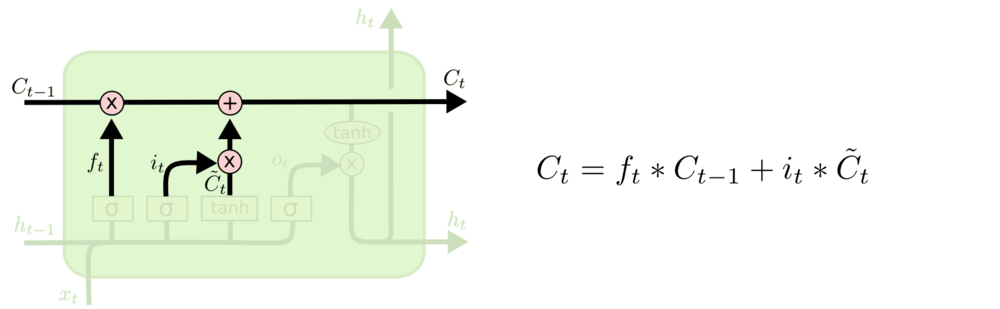
\includegraphics[width=1\textwidth]{./Tex_files/lstmcell.png}
			\caption{LSTM输入门}
		\end{figure}
		\item 输出门
		最后我们需要确定输出什么值,这个输出将会基于我们的细胞状态。首先,我们运行一个sigmoid层来确定细胞状态的哪个部分将输出出去。接着,我们把细胞状态通过 tanh进行处理(得到一个在 -1 到 1 之间的值)并将它和sigmoid门的输出相乘,最终我们仅仅会输出我们确定输出的那部分。
		\begin{figure}[h]
			\centering
			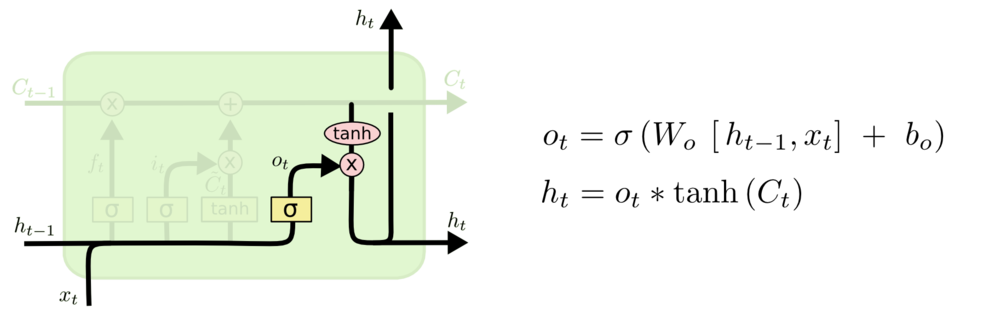
\includegraphics[width=1\textwidth]{./Tex_files/lstmoutput.png}
			\caption{LSTM输出门}
		\end{figure}
		\end{enumerate}
		\item 为什么LSTM可以解决梯度消失?
		Gradient Vanish的本质原因是矩阵高次幂导致的。\\
		使用一个合适激活函数,它的梯度在一个合理的范围。LSTM使用gate function,有选择的让一部分信息通过。gate是由一个sigmoid单元和一个逐点乘积操作组成,sigmoid单元输出1或0,用来判断通过还是阻止,然后训练这些gate的组合。所以,当gate是打开的(梯度接近于1),梯度就不会vanish。并且sigmoid不超过1,那么梯度也不会explode。
		\item 梯度裁剪
		\begin{figure}[h]
			\centering
			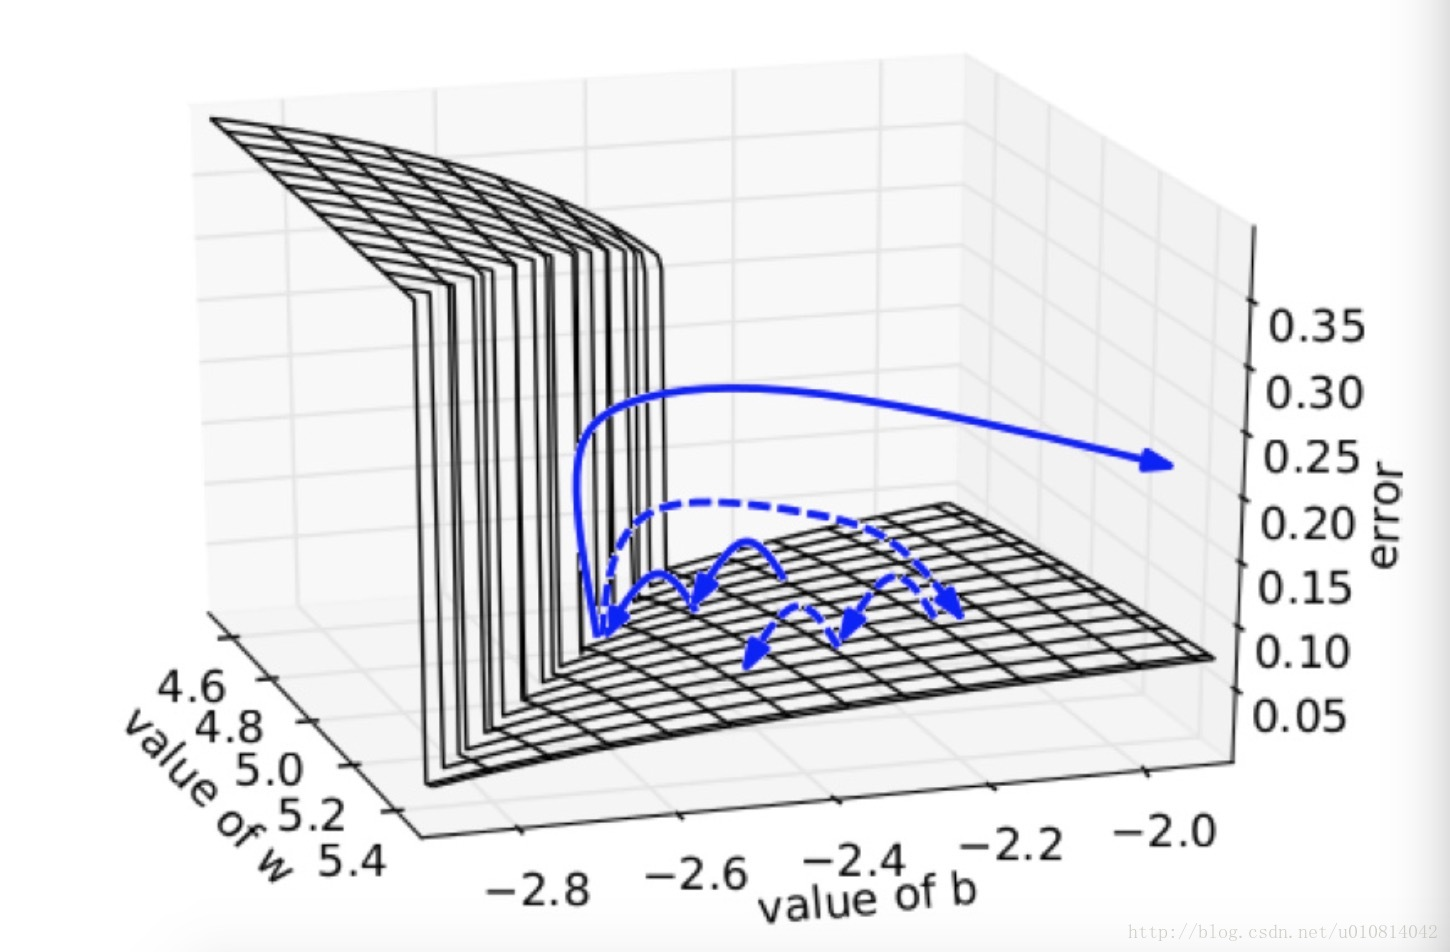
\includegraphics[width=1\textwidth]{./Tex_files/gradientclipping.png}
			\caption{梯度裁剪}
		\end{figure}
		\begin{itemize}
			\item 首先设置一个梯度阈值: clip\_gradient
			\item 在后向传播中求出各参数的梯度,这里我们不直接使用梯度进去参数更新,我们求这些梯度的l2范数
			\item 然后比较梯度的l2范数$||g||$与clip\_gradient的大小
			\item 如果前者大,求缩放因子clip\_gradient\/||g||, 由缩放因子可以看出梯度越大,则缩放因子越小,这样便很好地控制了梯度的范围
			\item 最后将梯度乘上缩放因子便得到最后所需的梯度 
		\end{itemize}
		\item GRU
		它是 LSTM 的简化版本,但在大多数任务中其表现与 LSTM 不相伯仲,因此也成为了常用的 RNN 算法之一。门控制循环单元(gated recurrent unit,GRU)网络是另一种基于门控制的循环神经网络,GRU的网络结构相比LSTM要简单一些。GRU将LSTM中的输入门和遗忘门合并成了一个门,称为更新门(update gate)。在GRU网络中,没有LSTM网络中的内部状态和外部状态的划分,而是通过直接在当前网络的状态
		\begin{figure}[h]
			\centering
			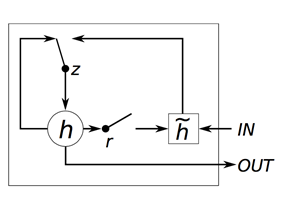
\includegraphics[width=0.8\textwidth]{./Tex_files/gru1.png}
			\caption{LSTM输出门}
		\end{figure}
		其中,r,z分别被称为 Reset Gate 和 Update Gate。可以看出,GRU 与 LSTM 有一定的相似性,而区别主要在于:
		\begin{enumerate}
			\item LSTM 有三个 Gate,而 GRU 仅两个
			\item GRU 没有 LSTM 中的 Cell,而是直接计算输出
			\item GRU 中的 Update Gate 类似于 LSTM 中 Input Gate 和 Forget Gate 的融合;而观察它们结构中与上一时刻相连的 Gate,就能看出 LSTM 中的 Forget Gate 其实分裂成了 GRU 中的 Update Gate 和 Reset Gate
		\end{enumerate}		
		很多实验都表明 GRU 跟 LSTM 的效果差不多,而 GRU 有更少的参数,因此相对容易训练且过拟合的问题要轻一点,在训练数据较少时可以试试。
	
\end{enumerate}
